\chapter{Conclusions}

In this report we have presented the Kalman filter we used for our robot. Now we will report an evaluation test on the accuracy af the filter with respect to the odometries calculated using sensors individually.\\

We drove the robot along the following trajectory starting and ending at point A and passing through the other points in the order B, C, D, E ,F.
\begin{figure}[!ht]
	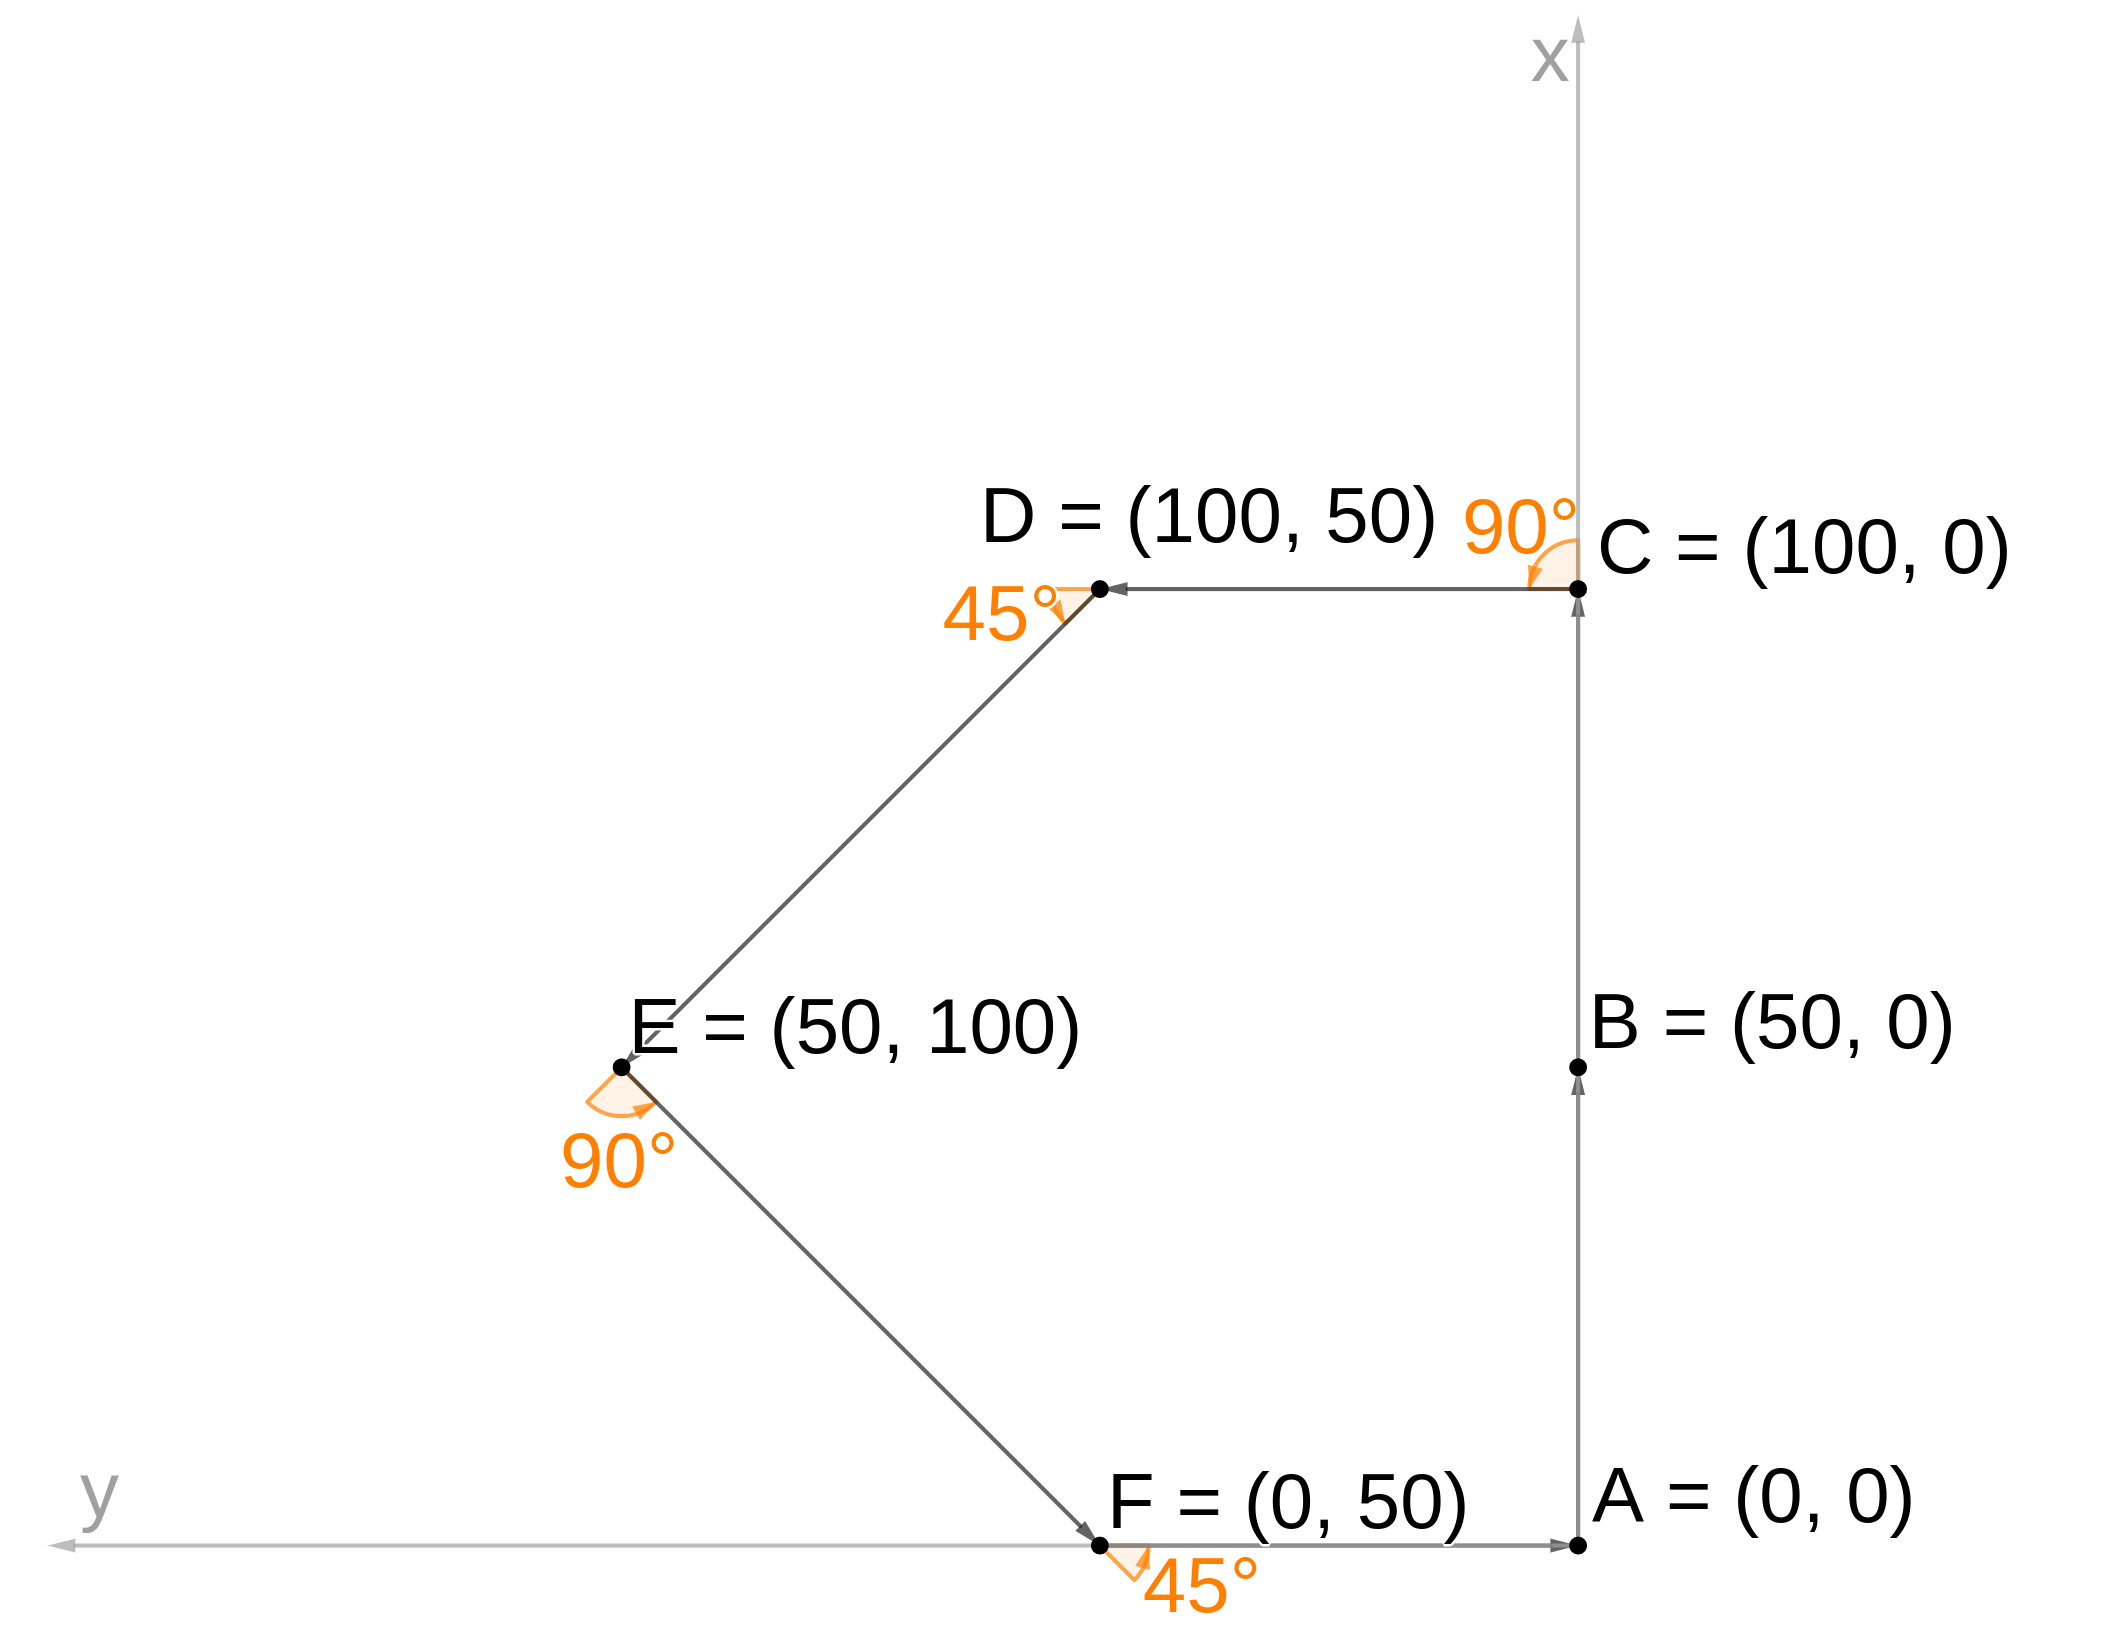
\includegraphics[scale=0.06]{test_path}
	\captionsetup{justification=centering, margin=1.5cm}
	\centering
	\caption{Expected trajectory for the test (distances are expressed in cm).}
	\centering
\end{figure}

\paragraph{Test 1}\mbox{}\\
\begin{figure}[!ht]
	\begin{subfigure}{0.35\textwidth}
		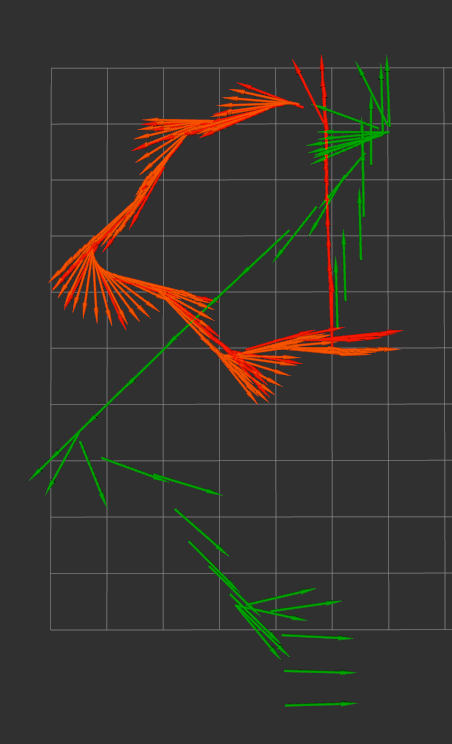
\includegraphics[width=\linewidth]{kf_test20}
	\end{subfigure}\hfil
	\begin{subfigure}{0.55\textwidth}
		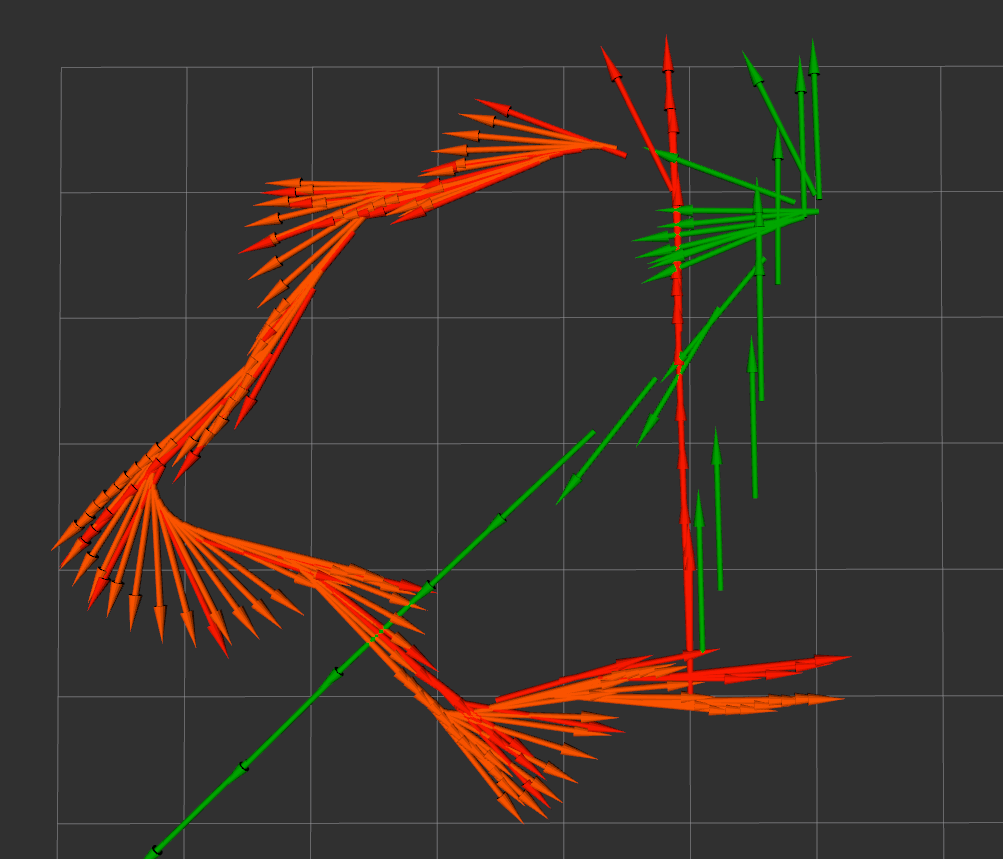
\includegraphics[width=\linewidth]{kf_test20_zoom}
	\end{subfigure}
	\captionsetup{justification=centering, margin=1.5cm}
	\centering
	\caption{Test 1 : estimated trajectories, Kalman filter trajectory in orange, Differential Drive trajectory in red, Inertial Navigation trajectory in green (visualized using RViz).}
	\centering
\end{figure}
\begin{table}[ht!]
	\centering
	\hspace*{-1cm}
	\begin{tabular}{rcccc}
		\toprule
		& \textbf{Expected} & \textbf{Kalman} & \textbf{Differential} & \textbf{Inertial}\\
		& \textbf{Position} & \textbf{Filter} & \textbf{Drive} & \textbf{Navigation}\\
		\midrule
		\textbf{A} & (0.000, 0.000, 0.000) & (0.000, 0.000, 0.000) & (0.000, 0.000, 0.000) & (0.000, 0.000, 0.000)\\
		\textbf{B} & (0.500, 0.000, 0.000) & (0.501, 0.009, 0.011) & (0.498, 0.016, 0.022) & (0.679, -0.141, 0.011)\\
		\textbf{C} & (1.000, 0.000, 0.000) & (1.002, 0.017, 0.010) & (0.999, 0.029, 0.011) & (0.991, -0.252, 0.010)\\
		\textbf{D} & (1.000, 0.500, 1.571) & (1.012, 0.523, 1.552) & (1.001, 0.534, 1.566) & (0.960, -0.256, 1.567)\\
		\textbf{E} & (0.500, 1.000, 2.356) & (0.509, 1.031, 2.325) & (0.481, 1.026, 2.349) & (-0.364, 1.117, 2.344)\\
		\textbf{F} & (0.000, 0.500, 3.927) & (-0.012, 0.518, 3.840) & (0.001, 0.479, 3.915) & (-1.136, 0.433, 3.866)\\
		\textbf{A} & (0.000, 0.000, 4.712) & (-0.009, 0.017, 4.721) & (0.046, -0.020, 4.807) & (-1.923, 0.205, 4.762)\\
		\bottomrule
	\end{tabular}
	\hspace*{-1cm}
	\caption{Test 1 : values for all the localization techniques [expressed as (x, y, theta)].}
\end{table}

By way of example we also report the final state\footnote{The state is expressed in the form $\begin{pmatrix}x & \dot{x} & \ddot{x} & y & \dot{y} & \ddot{y} & \theta & \dot{\theta}\\\end{pmatrix}\nonumber\\$} and covariance, calculated by the Kalman filter, at the end of the path after 60 seconds of motionless.
\begin{adjustwidth}{-0.6cm}{10pt}
	\begin{align}
		x &= \begin{pmatrix}
				-8.78e^{-3} & -1.14e^{-2} & -1.33e^{-2} & 1.67e^{-2} & 1.05e^{-2} & 1.24e^{-2} & 4.71 & -9.31e^{-4}\\
				\end{pmatrix}\nonumber\\
		\nonumber\\
		\Sigma_x &= \begin{pmatrix}
					2.67e^{-2} & 9.80e^{-5} & -2.37e^{-6} & 0 & 0 & 0 & 0 & 0\\
					9.80e^{-5} & 2.01e^{-4} & 2.34e^{-4} & 0 & 0 & 0 & 0 & 0\\
					-2.37e^{-6} & 2.34e^{-4} & 6.42e^{-4} & 0 & 0 & 0 & 0 & 0\\
					0 & 0 & 0 & 2.67e^{-2} & 1.00e^{-4} & 1.07e^{-8} & 0 & 0\\
					0 & 0 & 0 & 1.00e^{-4} & 2.06e^{-4} & 2.41e^{-4} & 0 & 0\\
					0 & 0 & 0 & 1.08e^{-8} & 2.41e^{-4} & 6.52e^{-4} & 0 & 0\\
					0 & 0 & 0 & 0 & 0 & 0 & 2.69e^{-7} & 2.51e^{-7}\\
					0 & 0 & 0 & 0 & 0 & 0 & 2.51e^{-7} & 5.01e^{-5}\\
				\end{pmatrix}\nonumber
	\end{align}
\end{adjustwidth}

\vspace{80pt}
\paragraph{Test 2}\mbox{}\\
\begin{figure}[!ht]
	\begin{subfigure}{0.35\textwidth}
		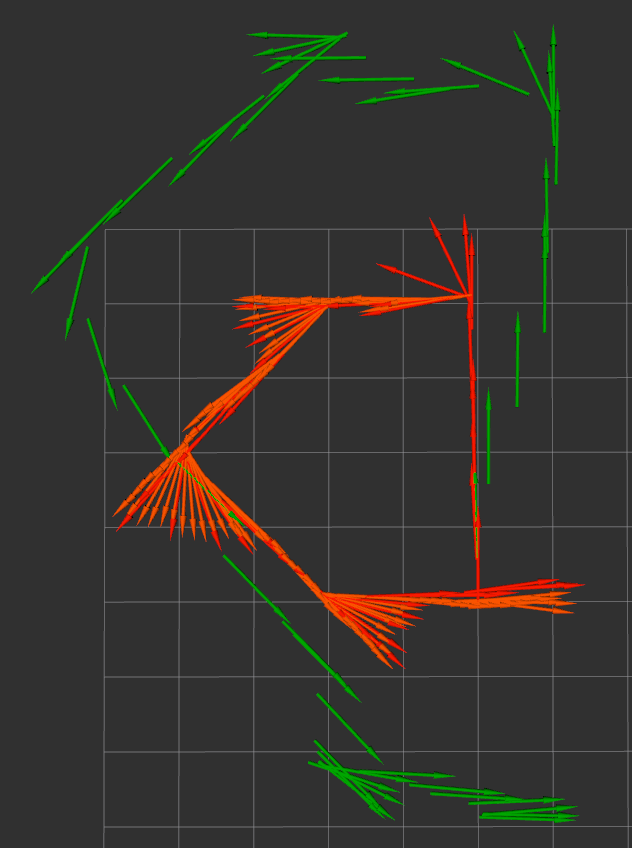
\includegraphics[width=\linewidth]{kf_test26}
	\end{subfigure}\hfil
	\begin{subfigure}{0.55\textwidth}
		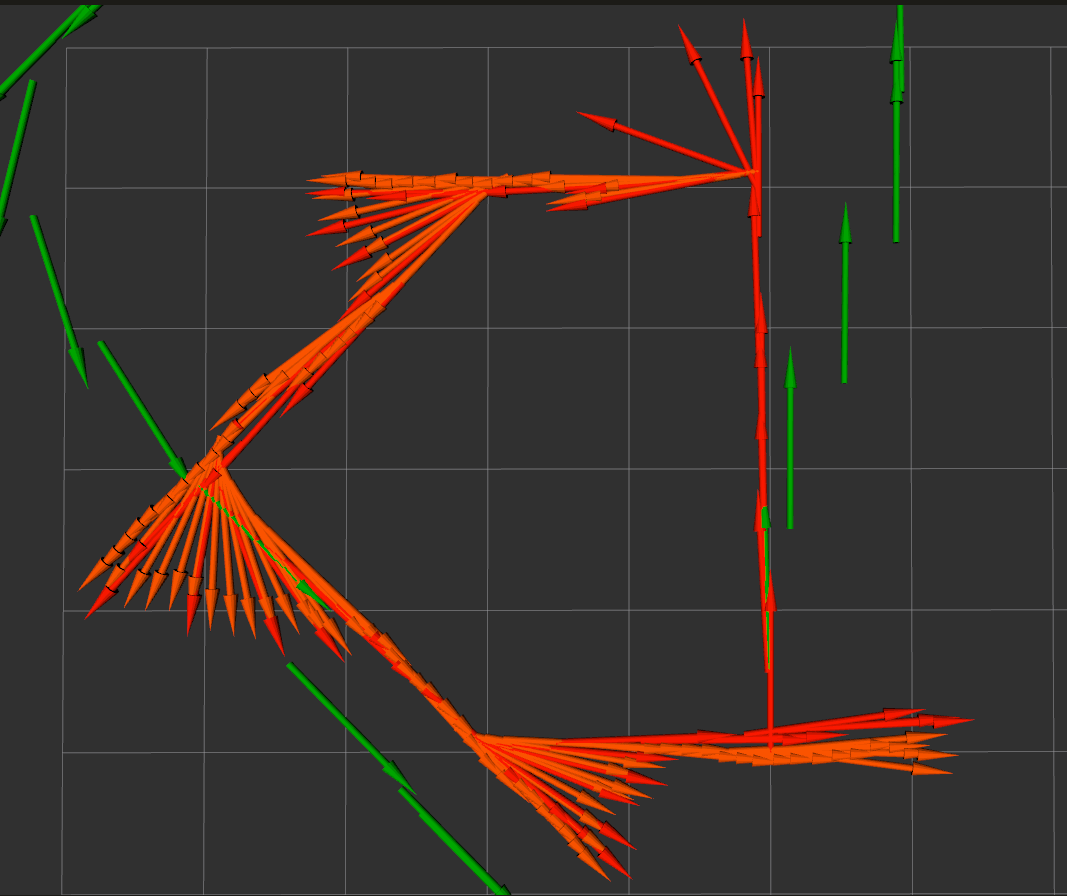
\includegraphics[width=\linewidth]{kf_test26_zoom}
	\end{subfigure}
	\captionsetup{justification=centering, margin=1.5cm}
	\centering
	\caption{Test 2 : estimated trajectories, Kalman filter trajectory in orange, Differential Drive trajectory in red, Inertial Navigation trajectory in green (visualized using RViz).}
	\centering
\end{figure}
\begin{table}[ht!]
	\centering
	\hspace*{-1.4cm}
	\begin{tabular}{rcccc}
		\toprule
		& \textbf{Expected} & \textbf{Kalman} & \textbf{Differential} & \textbf{Inertial}\\
		& \textbf{Position} & \textbf{Filter} & \textbf{Drive} & \textbf{Navigation}\\
		\midrule
		\textbf{A} & (0.000, 0.000, 0.000) & (0.000, 0.000, 0.000) & (0.000, 0.000, 0.000) & (0.000, 0.000, 0.000)\\
		\textbf{B} & (0.500, 0.000, 0.000) & (0.499, 0.000, 0.007) & (0.498, 0.012, 0.021) & (0.973, -0.224, -0.002)\\
		\textbf{C} & (1.000, 0.000, 0.000) & (1.001, 0.000, 0.006) & (0.980, 0.021, 0.076) & (1.528, -0.258, 0.056)\\
		\textbf{D} & (1.000, 0.500, 1.571) & (1.010, 0.501, 1.558) & (0.992, 0.502, 1.577) & (1.896, 0.455, 1.539)\\
		\textbf{E} & (0.500, 1.000, 2.356) & (0.516, 0.973, 2.348) & (0.524, 0.975, 2.367) & (-0.364, 1.117, 2.324)\\
		\textbf{F} & (0.000, 0.500, 3.927) & (0.006, 0.506, 3.906) & (-0.005, 0.481, 3.969) & (-0.516, 0.531, 3.911)\\
		\textbf{A} & (0.000, 0.000, 4.712) & (0.003, 0.000, 4.693) & (0.038, -0.025, 4.785) & (-0.707, -0.013, 4.691)\\
		\bottomrule
	\end{tabular}
	\hspace*{-1.4cm}
	\caption{Test 2 : values for all the localization techniques [expressed as (x, y, theta)].}
\end{table}
\newpage
By way of example we also report the final state and covariance, calculated by the Kalman filter, at the end of the path after 60 seconds of motionless.
\begin{adjustwidth}{-0.6cm}{10pt}
	\begin{align}
		x &= \begin{pmatrix}
				3.67e^{-3} & -3.57e^{-3} & -7.78e^{-3} & -2.38e^{-3} & 3.45e^{-3} & 7.69e^{-3} & 4.66 & 1.44e^{-4}\\
				\end{pmatrix}\nonumber\\
		\nonumber\\
		\Sigma_x &= \begin{pmatrix}
					1.31e^{-3} & 9.60e^{-6} & -8.84e^{-7} & 0 & 0 & 0 & 0 & 0\\
					9.60e^{-6} & 3.99e^{-5} & 8.70e^{-5} & 0 & 0 & 0 & 0 & 0\\
					-8.84e^{-7} & 8.70e^{-5} & 4.07e^{-4} & 0 & 0 & 0 & 0 & 0\\
					0 & 0 & 0 & 1.31e^{-3} & 9.60e^{6} & -8.84e^{-7} & 0 & 0\\
					0 & 0 & 0 & 9.60e^{-6} & 3.99e^{-5} & 8.70e^{-5} & 0 & 0\\
					0 & 0 & 0 & -8.84e^{-7} & 8.70e^{-5} & 6.52e^{-4} & 0 & 0\\
					0 & 0 & 0 & 0 & 0 & 0 & 1.31e^{-6} & 5.1e^{-9}\\
					0 & 0 & 0 & 0 & 0 & 0 & 5.1e^{-9} & 9.81e^{-7}\\
				\end{pmatrix}\nonumber
	\end{align}
\end{adjustwidth}
\vspace{80pt}
From these tests it emerges how the trajectory obtained with the sensor fusion (implemented through Kalman filtering) is surely far more accurate than the Inertial Navigation trajectory and it is also more accurate than the Differential Drive one. Moreover it also emerges how after a period of motionless the state is stable and the filter is very confident.\\

